% !TEX encoding = UTF-8 Unicode
\documentclass[a4paper,12pt]{article}
\usepackage{graphicx}
\usepackage{CJK}

\begin{CJK}{UTF8}{gbsn}

	\title{个人简历}
	\author{罗晓俊}

\end{CJK}

\begin{document}
	\begin{CJK}{UTF8}{gbsn}

		\maketitle{}

		% 照片
		\begin{figure}[h]
			\centering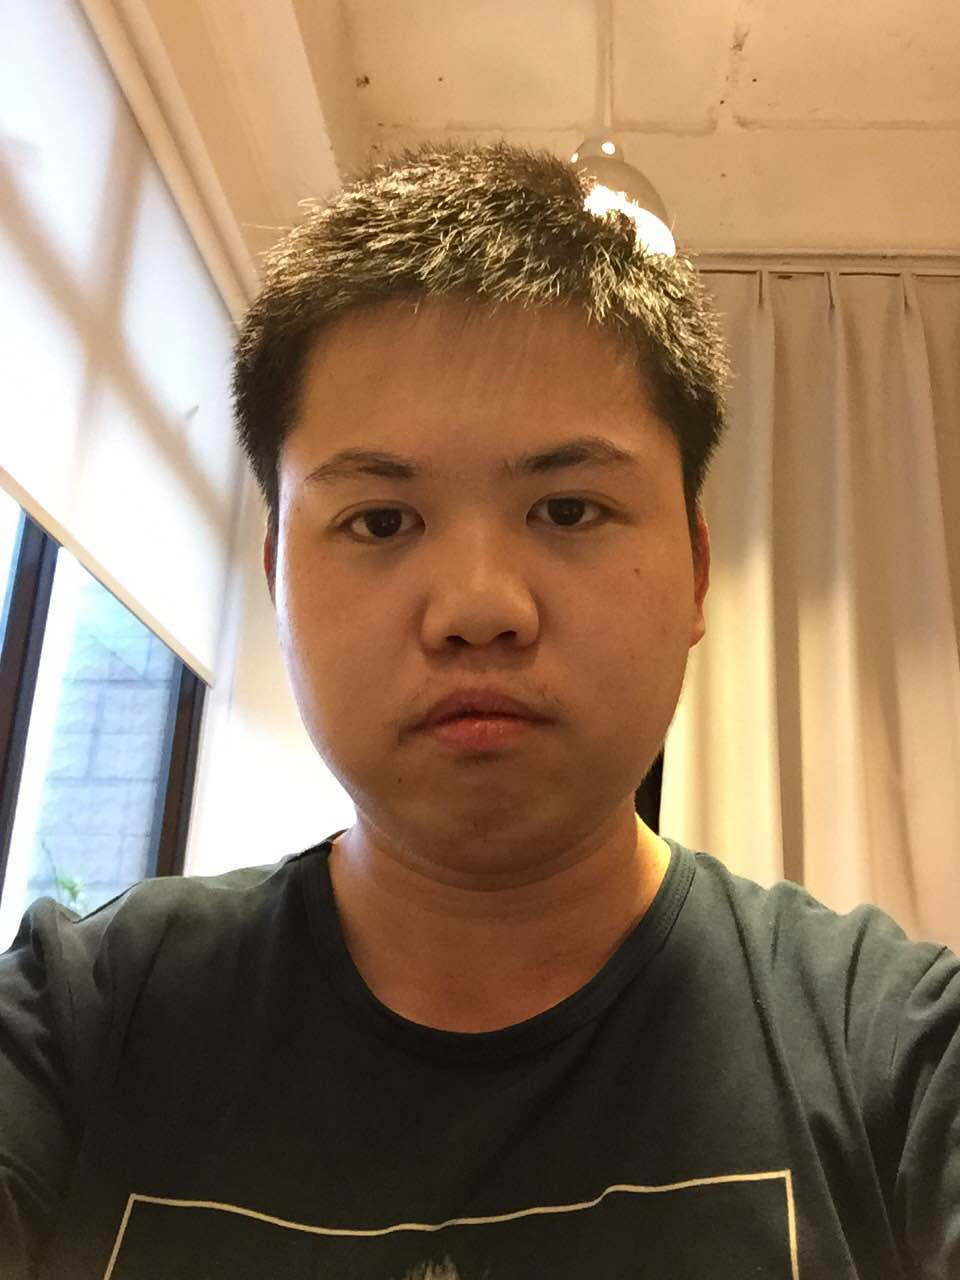
\includegraphics[height=100px]{webwxgetmsgimg.jpeg}
		\end{figure}

		% 个人简介
		\section{个人简介}
			崇尚极客精神,乐于学习和钻研技术,业余参与开源。
		
		% 教育经历
		\section{教育经历}
			\begin{itemize}
				\item{南昌工程学院 电气工程及其自动化 全日制本科 2014年毕业}
			\end{itemize}
		
		% 工作经历
		\section{工作经历}
			\begin{itemize}
				\item{2014.1 - 2015.10 融锋网络科技(上海)有限公司}
				\item{2015.11 - 2016.7 上海雀夸网络科技有限公司}
				\item{2016.7 - 2016.12 上海安个家信息技术有限公司}
				\item{2017.1 - 至今 上海乾升乾金融信息服务有限公司}
			\end{itemize}
		
		% 专业技能
		\section{专业技能}
			\begin{itemize}
				\item{熟悉PHP语言}
				\item{熟悉Linux、Mac开发环境}
				\item(熟悉MySQL使用)
				\item(熟悉Yii、Laravel、ThinkPHP框架)
				\item(了解HTTP、TCP/IP协议)
				\item(了解MySQL原理)
				\item(了解PHP内核原理)
			\end{itemize}
		
		% 项目经验
		\section{项目经验}
			\begin{itemize}
				\item{test1}
				\item{test2}
			\end{itemize}
		
		% 开源贡献
		\section{开源贡献}
		 	\begin{itemize}
				\item{GitHub: https://github.com/luoxiaojun1992}
				\item{test2}
			\end{itemize}	

	\end{CJK}
\end{document}
